

\chapter{Novel methodology for damage detection}\label{methodology}

In this chapter of~the~dissertation, author presents the~methodology developed and applied towards simulated and real signals. The elementary techniques of~these methods are known and used in~other areas of~research. However, the~novelty of~this dissertation lies in~designing specific analytical methods utilizing said techniques, that can successfully deal with the~difficulties related to~the~diagnostics of~heavy-duty mining machinery.

\section{Methods for temperature data analysis for technical condition change detection}\label{temps}

Temperature data can be~a~very rich source of~diagnostic information. While being very natural to~understand, its meaning is~also universal across numerous types of~machines. Hence, in~this chapter methods \ref{temp_ica} and \ref{temp_em} regard the~analysis of~temperature data recorded on~the~belt conveyor gearboxes, and on~the~other hand techniques \ref{temp_bulgaria} and \ref{temp_ad} consider temperature data measured on~the~LHDs. 

\subsection{Failure detection using ICA}\label{temp_ica}

In this section, author presents the~first method developed for real-life temperature signals from the~set of~four heavy duty gearboxes of~a~single belt conveyor driving station used in~the~mining industry. Many times in~the~literature it~has been proven that for condition monitoring, especially in~the~context of~spatially distributed information, taking advantage of~multichannel data can be~very beneficial in~the~context of~removing environmental influence, but also integrating the~informativeness scattered across the~channels. Following this idea, it~was proposed to~develop a~diagnostic procedure that uses Independent Component Analysis (ICA) as~a~tool for extracting the~damage-related information hidden in~the~four-channel signal. 

\begin{figure}[ht!]
\centering
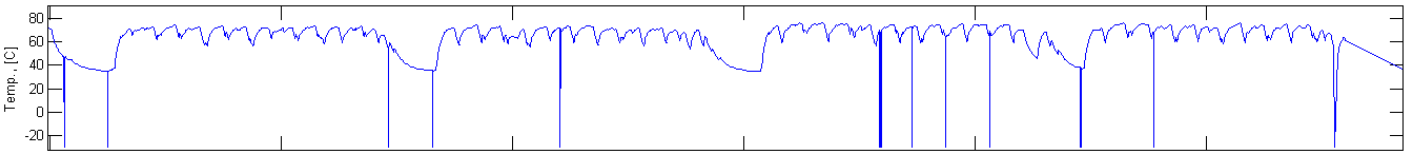
\includegraphics[width = \textwidth]{wykresy/ex_temp.PNG}
\caption{Example of~raw temperature data.}
\label{fig: ex_temp}
\end{figure}

In the~first step, the~outliers have been removed from the~data. In this case outliers are values lower than $0$. This effect in~the~signal is~considered to~be acquisition error since such values are forbidden by~the~physics of~the~process. Removed values have been replaced using local linear interpolation, which in~practice is~equivalent to~the~mean value of~the~neighboring samples (see Eq. \ref{eq:interp}).

\begin{equation}\label{eq:interp}
  x_{i}=\frac{x_{i-1}+x_{i+1}}{2} \quad \forall i: x_i<0
\end{equation}

The SCADA system that registered this data reacts to~the~value changing by~at~least predefined $\Delta T$, in~this case, equal to~1 degree Celsius. This approach allows reducing the~number of~recorded samples because repeating values are not stored. Linear interpolation is~the~simplest, yet best-suited method for interpolating such variables because, by~definition, the~intermediate sample can only take the~value between the~two existing neighbors. Unfortunately, the~described acquisition method makes the~data not evenly sampled, so after that, the~resampling was performed with output sampling period fixed to~15 minutes. To achieve that goal author used built-in Matlab function \code{resample}. 

After the~preprocessing, ICA was used to~separate the~intrinsic information sources in~the~dataset, which effectively allowed to~extract the~information indicating the~variation in~the~technical condition of~one of~the~gearboxes. In practice, four output variables are produced, that are called \emph{independent components} of~the~dataset. One of~those is~expected to~contain the~damage-indicating information. A~detailed description of~used ICA algorithm can be~found in~the~appendix in~section \ref{app_ica}.

When the~independent components are obtained, for each of~them algorithm searches for an~index $ind$ in~the~time domain that divides the~component into two parts that have the~highest possible difference in~the~mean value (see Eq. \ref{eq:divind}). 

\begin{equation}\label{eq:divind}
  ind=\argmaxB_i(\mathrm{abs}(\mathrm{mean}(x[1:i])-\mathrm{mean}(x[i+1:end])))
\end{equation}

Then, the~component characterized by~the~highest difference of~means is~identified as~the~component of~interest. Cross-correlating this component with all original channels allows determining which of~the~gearboxes the~misbehavior is~coming from. Correlation coefficients for this evaluation have been calculated using built-in Matlab function \code{corrcoef}. 


Finally, the~selected feature is~segmented into individual days based on~known sampling parameters. For each day, the~squared variance $vs^{(D)}$ is~calculated for each day $D=\{1,2,...,N\}$ where N is~the~number of~days in~the~data set. 

\begin{equation}\label{eq:divind2}
  vs^{(D)}=\left(\frac{1}{n}\sum^n_{i=1}\left(x_i^{(D)}-\mu^{(D)} \right)\right)^2,
\end{equation}
where $x^{(D)}$ is~segment of~a~particular day, $n$ is~its length and $\mu^{(D)}$ is~its mean value. 

Obtained vector $vs$ is~thresholded based on~its mean value $thr=mean(vs)$. The day where $vs>thr$ is~when the~overheating began. Functional flowchart of~the~procedure is~presented in~Figure \ref{fig: sch_ica}. The~procedure has been published in~\cite{wodecki2017application}.

\begin{figure}[ht!]
\centering
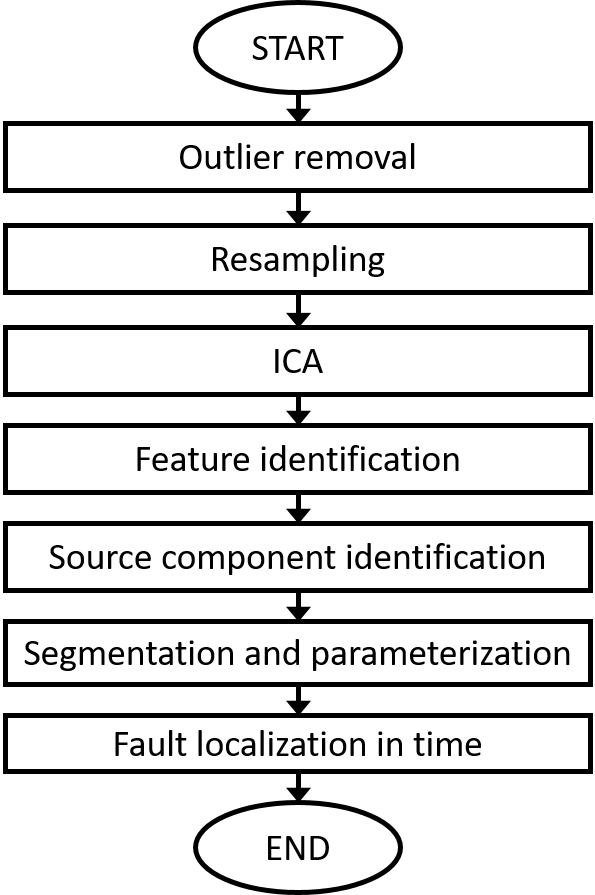
\includegraphics[width = 0.4\textwidth]{wykresy/sch_ica.png}
\caption{Flowchart of~proposed procedure.}
\label{fig: sch_ica}
\end{figure}

\subsection{Work regimes distinction using EM}\label{temp_em}

In this section the~methodology using the~clustering method was developed for the~long-term observations of~the~temperature in~order to~detect gearbox fault, that manifests itself as~a~non-typical behavior of~the~temperature data. The algorithm also identifies the~specific character of~the~work at~the~beginning and end of~the~week. For this methodology author analyzes temperature data acquired by~commercial, multichannel low-frequency data logger installed on~the~belt conveyor gearboxes in~a~copper ore mine.

Before starting any data analysis one should be~sure that the~data was acquired properly and the~incorrect values were removed, which allows to~avoid coming to~the~false conclusions of~the~analysis. The pre-processing procedures are obligatory in~case of~temperature data from belt conveyor gearbox. Author applied two-step procedure: data cleaning and resampling performed in~the~same way as~described in~section \ref{temp_ica}. The data after application of~pre-processing procedures is~shown in~Fig. \ref{fig: L222_55_data}.

\begin{figure}[ht!]
\centering
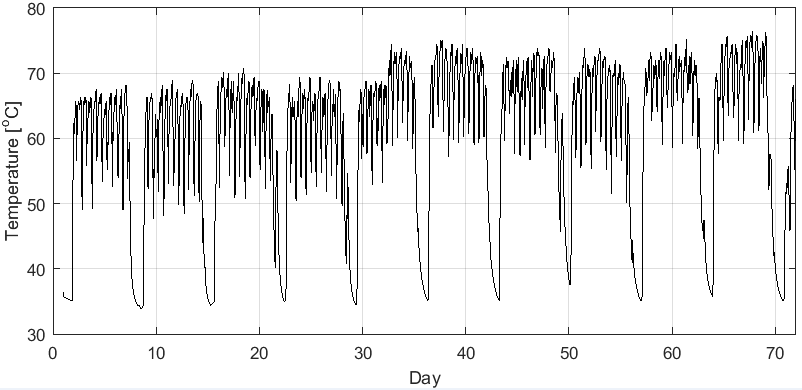
\includegraphics[width = 1\textwidth]{wykresy/L222_55_data.png}
\caption{Real temperature data from belt conveyor gearbox after pre-processing.}
\label{fig: L222_55_data}
\end{figure}

As one can see, visible cyclic drops of~the~temperature value are present. They are connected to~the~weekend periods when the~conveyor is~not operating. In that time the~gearbox is~cooled down to~the~ambient temperature. That specific behavior allows to~easily split the~data into segments corresponding to~each week of~the~belt conveyor operation. Moreover one can notice that at~$33$rd day of~collected data the~sudden increase in~the~temperature value occurs. Values of~temperature remain elevated for a~long time. The increase of~temperature is~a~symptom of~a~change of~technical condition of~a~machine. Therefore the~aim of~the~work is~to~propose an~anomaly detection procedure, which automatically indicates the~alarming time point.

Using the~time information, pre-processed data was segmented into sub-signals related to~one day of~a~belt conveyor operation. In Fig. \ref{fig: L222_55_days} one can see a~difference between the~behavior of~examined data depending on~the~day of~the~week. It should be~mentioned that in~the~copper ore mine there is~a~four shift work system. Moreover, on~Saturday the~work finishes at~6 p.m. and then begins at~6 a.m. on~Monday. Therefore, during the~$36$-hour stoppage in~operation, the~belt conveyor is~cooled down to~the~ambient temperature. This time period is~used for planned maintenance tasks. In other days the~cyclic breaks in~working are caused by~blasting procedures, which in~copper ore mine are performed twice during the~day. It is~reflected in~the~time series as~two temperature local minima about $9$ a.m. and $9$ p.m. Such behavior of~data can be~the~indicator in~the~clustering process, which is~used to~recognize working days when the~overheating takes place.

\begin{figure}[ht!]
\centering
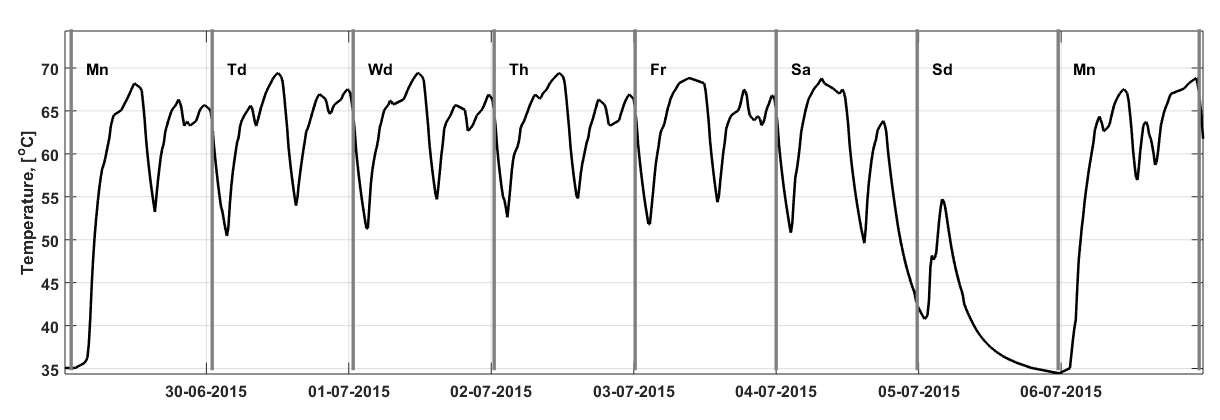
\includegraphics[width = \textwidth]{wykresy/days.png}
\caption{Behavior of~the~temperature time series depending on~day of~the~week.}
\label{fig: L222_55_days}
\end{figure}

The clustering procedure used for unsupervised anomaly detection is~the~Expectation-Maximization algorithm, described in~detail in~the~appendix in~section \ref{EM}. Statistics used to~feed the~clustering algorithm were simple, yet informative:

\begin{itemize}
\renewcommand{\labelitemi}{$\bullet$}
\item Maximum value of~the~day, 
\item Dispersion of~values of~the~day,
\item Value at~the~end of~the~day,
\end{itemize}
more formally:

\begin{equation}
  \chi=\left[\max(x), \max(x)-\min(x), x_{end} \right]
\end{equation}

The~three-dimensional feature vector of~described statistics has been constructed in~the~time domain for each day. Clustering of~this vector in~three dimensions using the~Expectation-Maximization algorithm (see section \ref{EM}) allowed to~classify the~days, and identify those revealing the~anomalous behavior. Functional flowchart of~the~procedure is~presented in~Figure \ref{fig: sch_em}. The~procedure has been published in~\cite{wodecki2018unsupervised}.

\begin{figure}[ht!]
\centering
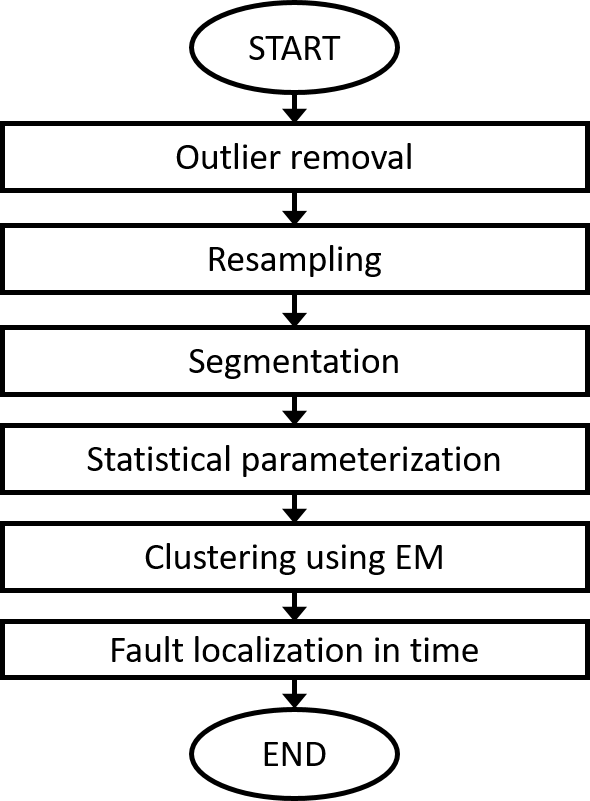
\includegraphics[width = 0.4\textwidth]{wykresy/sch_em.png}
\caption{Flowchart of~proposed procedure.}
\label{fig: sch_em}
\end{figure}


\subsection{Time-time map analysis for LHD fault detection}\label{temp_bulgaria}

In this section, the~author addresses the~subject of~long-term analysis of~LHD's engine coolant temperature data in~order to~identify the~abnormal behavior, impossible to~be noticed having only short-term section of~the~data. 

Instantaneous value of~the~temperature is~influenced by~many factors, such as~workload, ambient temperature, restrictions in~heat exchange with the~air (e.g. when cooler is~close to~the~wall or is~plastered with mud), overall temporal efficiency of~the~cooling system, etc. It is~crucial to~understand that all of~the~factors can vary in~time. That amount of~varying parameters makes short-time temperature data analysis very difficult. As a~solution to~this problem author proposes to~perform a~long-term analysis, which allows reducing the influence of~fast-changing factors like varying workload during a~single work shift, temporary difficulties with heat exchange or variations of~ambient temperature. In such case, it~is~assumed that relevant temperature changes will be~connected mainly with the~technical condition of~the~machine.

Statistical approach used in~this methodology allows for looking at~the~data in~more aggregated way than only as~a~raw time series (see section \ref{prep}) \cite{sikora2012regime,wylomanska2014signal,azami2012improved,rathi2006seeing,wylomanska2012identify}. Proposed method considers work shifts as~integral parts of~data and investigates their kernel density estimate functions (see section \ref{param}). Work performed by~the~LHD is~mainly transport of~ore from the~mining face to~the~dumping point, so in~the~long run character of~this task is~mostly consistent. Hence, temperature distribution from shift to~shift should be~similar. However, in~case of~change of~technical condition of~the~machine (failure, repair and such) we expect a~significant change of~density function to~happen. This change can regard not only the~shift of~whole distribution function towards higher or lower values but the~change of~the~dispersion of~values as~well. To identify those changes the~author proposes to~define diagnostic parameters that are selected based on~the~observation of~data behavior. Parameters are expected to~reveal sudden changes in~the~data representation and ease of~their analysis will result in~a~very practical way of~health condition changes identification.

\subsubsection{Preprocessing}\label{prep}

LHD machines operate in~highly time-varying environmental conditions in~the~underground mine. Changing load and variability of~tasks lead to~different amounts of~data and its varying quality. Because of~those difficulties, the~proper selection of~data has to~be performed. The~important issue with the~original record is~a~substantial amount of~missing data points. Since the~approach is~shift-oriented, the~first task is~to~eliminate shifts that have too much data absent. First, the~author proposes to~visualize data in~3D space where temperature $T$ is~represented in~the~domain of~local time $t$ describing the~time during one work shift, and $\Theta$ that is~long-term time indicating consecutive work shifts. It can be~rewritten as:

\begin{equation}
  T=f(t,\Theta)
\end{equation}

To extract the~usable part of~data, the~amount of~empty values for each shift is~counted and placed in~a~vector. After that, the~distribution density function of~the~obtained vector is~calculated. 

\begin{equation}
  \hat{f}_h(x)=\frac{1}{nh}\sum_{i=1}^n K\left(\frac{x-x_i}{h}\right),
\end{equation}
where $x_i$ are random samples from an~unknown distribution, $n$ is~the~sample size, $K(\cdot)$ is~the~kernel function and $h$ is~the~bandwidth.


The density function has two major modes representing shifts with much data missing, and shifts with only a~small amount of~data missing. The~local minimum of~density function between those modes indicates the~threshold value above which shifts are disregarded. 

\subsubsection{Parameterization}\label{param}

After selecting the~appropriate set of~shifts from the~initial data, the~probability density estimate function of~every shift is~calculated \cite{bowman1997applied}. Vectors of~function values for each shift are arranged into a~matrix that forms so-called probability density map. The map itself in~some way reveals the~behavior that we were looking for, but on~the~small scale consecutive distributions are quite inconsistent and parameterization is~difficult at~this point. To achieve a~more useful character of~the~map, we regard it~to~be an~image, and smooth it~using two-dimensional convolution filter:

\begin{equation}
  \hat{T}=T\circ M,
\end{equation}
where $\hat{T}$ is~the~filtered map $T$, $\circ$ is~the~convolution operator and $M$ is~a~quasi-Gaussian kernel:

\begin{equation}
M=\frac{1}{81}*
\begin{bmatrix}
  1 & 2 & 3 & 2 & 1 \\
  2 & 4 & 6 & 4 & 2 \\
  3 & 6 & 9 & 6 & 3 \\
  2 & 4 & 6 & 4 & 2 \\
  1 & 2 & 3 & 2 & 1 \\
\end{bmatrix}
\end{equation}
where division by~81 means normalizing the~kernel by~the~total sum of~its fields \cite{arce2005nonlinear}. Values of~the~kernel were selected experimentally. The~ordinary two-dimensional moving average would smooth the~map way too much, so the~bell curve was chosen for better selectiveness after the~filtration. It causes the~nearest samples to~have a~greater impact on~the~center sample and further samples to~have a~lesser impact. In practice, this operation slightly smooths the~sharp spikes and improves the~consistency within the~regimes that we want to~distinguish apart. It also allows for calculated statistics described in~the~next chapter to~take more consistent form.

\subsubsection{Statistics and event description}

Parameterization of~shifts will require data samples, but since density map has been modified it~means that data itself is~not the~same anymore, so we can’t use original temperature data any longer. The easiest way to~obtain data samples from new distributions is~to~draw them from the~inverse empirical cumulative density function estimates $\hat{C}$ created by~numerical integration of~the~smoothed probability density map $\hat{T}$ \cite{devroye1986sample} such as:

\begin{equation}
  \hat{C}_{(i,j)}=\sum_{k=1}^j \hat{T}_{(i,k)}
\end{equation}

When samples are obtained for each shift, the~vector of~interquartile ranges has been calculated. Interquartile range (IQR) is~defined as~a~measure of~statistical dispersion, being equal to~the~difference between the~upper and lower quartiles, such as:

\begin{equation}
  IQR_i=\overline{\left(\hat{C}_i^+\right)_{(J/2+1:J)}}- \overline{\left(\hat{C}_i^+\right)_{(1:J/2)}}
\end{equation}
where $(\cdot)^+$ means vector sorted in~the~ascending order, $\overline{(\cdot)}$ is~a~median operator and $J$ is~the~length of~$\hat{C}_i^+$ vector.

The~second statistic is~a~vector of~locations of~probability density map maxima for shifts, and it~can be~calculated directly from the~map. Each statistic is~expected to~indicate the~changes in~data occurring with respect to~the~global time $\Theta$. To identify timestamps of~those change points, in~each statistic we find a~point that splits the~statistic into two parts of~the~highest difference in~mean. Obtained points are expected to~allow to~localize regime changes in~time. The~procedure has been published in~\cite{wodecki2016condition}.

\subsection{Anderson-Darling statistic map for failure detection}\label{temp_ad}

In this section, the~author proposes to~use long-term temperature data analysis for evaluating changes in~a~technical condition connected to~engine overheating in~LHD machines. This method focuses on~developing an~alternative technique to~differentiate time segments containing data that describe different technical condition of~the~machine. Author takes advantage of~the~fact that the~statistical distribution of~temperature data differs according to~technical condition \cite{wodecki2016condition}. Appropriate transformation of~long-term temperature data and application of~Anderson–Darling (AD) statistic (see section \ref{met_ad}) allows quantifying those differences in~the~form of~a~two-dimensional map of~the~test statistic. Analysis of~this map results in~the~detection of~points where the~technical condition of~the~machine changes significantly.

Proposed method is~based on~long-term data observation. Based on~the~general assumption about the~way that overheating leads to~machine failure one can define three disjoint processes occurring consecutively:

\begin{itemize}
  \item[$\bullet$] \emph{Process 1:} Machine is~operating while in~bad technical condition, overheating significantly;
  \item[$\bullet$] \emph{Process 2:} Machine experiences a~cooling system failure, but is~still being operated;
  \item[$\bullet$] \emph{Process 3:} Failure is~repaired and machine operates in~good technical condition.
\end{itemize}

In such case one can describe those processes in~terms of~signal parameters:

\begin{itemize}
  \item[$\bullet$] \emph{Process 1:} High median, low variance (warning state approaching failure);
  \item[$\bullet$] \emph{Process 2:} High median, high variance (failure state);
  \item[$\bullet$] \emph{Process 3:} Low median, high variance (healthy state).
\end{itemize}

Despite the~relatively simple definition of~the~processes, it~is~not easy to~define one simple diagnostic criterion.

\subsubsection{Pre-processing}

Input data is~imported in~the~time domain, so pre-processing is~required. Firstly, non-overlapping six-hour segments of~the~signal that denotes six-hour work shifts, are framed into the~new matrix as~its columns. Then columns with an~excessive amount of~missing values are rejected based on~the~distribution of~their amount in~each column. Since remaining columns still contain small amounts of~missing values, they are interpolated using the~nearest-neighbour method. Such a~matrix representing the~temperature in~a~time-time domain is~ready for further analysis.

\subsubsection{Anderson-Darling statistic}\label{met_ad}

Because of~different behavior in~observed regimes (changing the~median and variance) the~author proposes to~calculate the~empirical cumulative distribution functions (ECDF) of~each work shift and compare statistic based on~distances between them. ECDF of~the~random variable $X$ can be~defined as:

\begin{equation}
  \hat{F}_n(t)=\frac{1}{n}\sum_{i=1}^n 1_{X_i\leq t}
\end{equation}
where $1_A$ is~the~indicator of~event $A$ and $n$ is~the~length of~realization of~$X$. 

Usually it~is~calculated in~supremum (Kolmogorov - Smirnov \cite{massey1951kolmogorov}) or quadratic (Cram{\'e}r - von Mises family \cite{laio2004cramer}) norm. For signal parameterization author proposes to~use statistic based on~quadratic norm between two ECDFs. Kolmogorov - Smirnov test is~widely recognized and used as~a~classical method, but AD test is~described in~the~literature as~more powerful and hence superior \cite{razali2011power,engmann2011comparing}. a~class of~measures of~discrepancy is~given by~Cram{\'e}r - von Mises family:

\begin{equation}
\label{one-sample_ad}
  Q^2=n \int\limits_{-\infty}^{\infty} \{F_n(x) - F(x) \}^2 \psi(x)dF(x)
\end{equation}
where $F_n(x)$ is~ECDF, $F(x)$ is~theoretical CDF that $F_n(x)$ is~compared to, $\psi(x)$ is~a~function of~weights. $\psi(x)=1$ gives $\omega^2$ statistic of~Cram{\'e}r - von Mises. To obtain Anderson - Darling statistic $A^2$ the~vector of~weights is~given by~$\psi(x)=[F(x)(1-F(x))]^{-1}$ \cite{pettitt1976two,cizek2005statistical}. In the~real data analysis the~integral in~formula \ref{two-sample_ad} reduces to~the~finite sum which corresponds to~the~distance between theoretical and empirical cumulative distribution functions in~appropriate norm.

In presented case author used two-sample Anderson - Darling statistic which is~modification of~(\ref{one-sample_ad}):

\begin{equation}
\label{two-sample_ad}
  A^2_{nm}=\frac{mn}{N} \int\limits_{-\infty}^{\infty} \frac{\{F^i_m(x) - F^j_n(x) \}^2} {H_N(x)(1-H_N(x))}dH_N(x),
\end{equation}
where $F^i_m$, $F^j_n$ are ECDFs of~$i^{th}$ and $j^{th}$ work shifts and $H_N$ with $N=n+m$ is~the~weight function, for $n$ and $m$ being the~number of~observations in~work shifts. The $H_N$ function is~given by~combining $F^i_m$ and $F^j_n$ distribution: $H_N(x)=\frac{mF^i_m(x)+nF^j_n(x)}{N}$. It is~used to~test hypothesis $F^i_m=F^j_n$. In presented method author calculates Anderson - Darling statistic defined by~(\ref{two-sample_ad}) for every pair of~shifts and construct 2D map of~values. The resulting map is~symmetric relative to~its main diagonal.

\subsubsection{Smoothing of~AD map}

After calculating the~map of~AD statistic, it~requires minor smoothing to~obtain more consistent levels in~distinctive areas of~the~map \cite{bowman1997applied}. The~author proposes to~use two-dimensional a~convolution-based filter with normalized triangular kernel \emph{K} based on~a~vector $v=\left[1,2,1 \right]$ (\ref{eq:kernel}). 
\begin{equation}
\label{eq:kernel}
K = \frac{v^T v}{\sum{\left(v^T v \right)}} = \frac{1}{\sum{\left(v^T v \right)}}\left[\begin{array}{ccc}1&2&1\\2&4&2\\1&2&1\end{array}\right] =
\left[\begin{array}{ccc}0.0625&0.125&0.0625\\0.125&0.25&0.125\\0.0625&0.125&0.0625\end{array}\right]
\end{equation}

\subsubsection{AD map analysis}

Considering knowledge about general behavior of~the~processes described in~previous sections, one can make a~few assumptions about the~expected structure of~AD map (see Fig. \ref{fig:map}):
\begin{enumerate}
\item ECDFs of~shifts within a~single process will be~similar, hence values of~AD statistic in~the~areas (1,1), (2,2) and (3,3) will be~relatively low, because those are the~areas where shifts of~a~given process are compared with shifts of~the~same process. 
\item ECDFs of~shifts from warning and failure processes are similar for failure shifts where the~machine was not cooled down on~purpose, and different for failure shifts where the~machine was purposely cooled down (regions (1,2) and (2,1)).
\item Analogous case occurs when comparing ECDFs of~shifts from failure and healthy process: they are similar for failure shifts where the~machine was purposely cooled down, and dissimilar otherwise (regions (2,3) and (3,2)).
\item Comparing warning and healthy processes, ECDFs are not similar at~all, hence those regions of~AD map will be~characterized with high values (regions (1,3) and (3,1)).
\end{enumerate}

\begin{figure}[ht!]
\centering
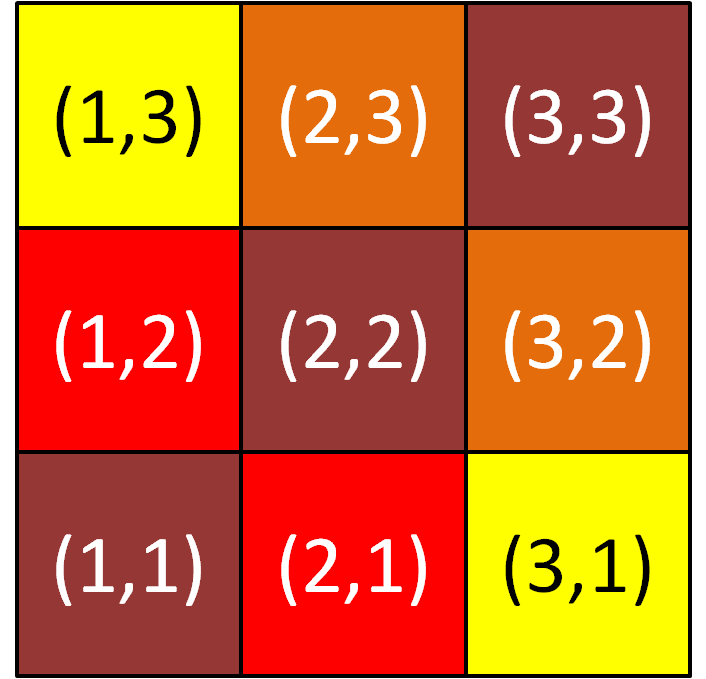
\includegraphics[width=0.5\textwidth]{wykresy/map.png}
\caption{Logical chart of~expected AD map}
\label{fig:map}
\end{figure}

It is~hard to~find transition points based on~two-dimensional data. Hence, the~author proposes to~determine the~threshold based on~one-dimensional statistic. Taking advantage of~previously mentioned assumptions, it~is~expected that the~variance of~AD map vectors will vary according to~the~area. Hence, in~a~next step one-dimensional sample variance of~the~smoothed map is~calculated. Since the~second process shares similar features with two remaining ones, which on~the~other hand are different from each other, one can expect certain behavior of~the~variance values of~particular groups of~AD map columns:

\begin{itemize}
\item[$\bullet$] \textbf{Group regarding process 1 (columns of~areas (1,x)):} relatively high variance values. AD statistic values will be~low when comparing process 1 to~itself, medium when comparing it~to~process 2 (similar median) and high when comparing it~to~process 3 (no similar parameters);
\item[$\bullet$] \textbf{Group regarding process 2 (columns of~areas (2,x)):} relatively low variance values. AD statistic values will be~low when comparing process 2 to~itself, and medium when comparing it~to~processes 1 and 3 (similar median or variance);
\item[$\bullet$] \textbf{Group regarding process 3 (columns of~areas (3,x)):} relatively high variance values. AD statistic values will be~low when comparing process 3 to~itself, medium when comparing it~to~process 2 (similar variance) and high when comparing it~to~process 1 (no similar parameters);
\end{itemize}

Based on~that assumption one could imagine that group 2 is~expected to~exhibit lower sample variance than groups 1 and 3. Hence, it~is~proposed to~threshold sample variance vector based on~the~histogram with bin width $BW$ calculated using Freedman-Diaconis rule defined as~\cite{freedman1981}:

\begin{equation}
  BW=2\frac{IQR(X)}{\sqrt[3]{n}},
\end{equation}
where $n$ is~a~number of~elements in~the~vector $X$.

Values describing group 2 are expected to~cluster around lower variance value than values describing groups 1 and 3, so a~natural local minimum is~expected to~appear on~the~histogram between group 2 and groups 1 and 3. Location of~that local minimum serves as~a~threshold that allows to~separate groups using the~variance vector as~a~feature, and hence to~find the~transition points between technical condition states. The~procedure has been published in~\cite{wodecki2017technical}.

\section{Muiltichannel spectrogram analysis using PCA}\label{met_pca}

A multichannel vibration data processing method in~the~context of~local damage detection in~gearboxes is~presented in~this section. The purpose of~the~approach is~to~achieve more reliable information about local damage when using several channels in~comparison to~results obtained for single-channel vibration signal. 

First, the~transformation of~$N$ input channels into time-frequency representations is~performed. For this purpose, a~spectrogram is~used according to~the~definition provided in~the~appendix (see section \ref{STFT}). As a~result, a~three-dimensional data structure is~created, such that:

\begin{equation}
  S^{(i\times M\times K)}=spec\left(X_i^{(1\times L)} \right),
\end{equation}
where $i=(1,\dots,N)$ is~the~number of~input channel, $L$ is~the~number of~samples in~each input channel, and $M\times K$ is~the~size of~calculated spectrograms in~frequency and time domain respectively.

In the~next step, the~time-frequency maps are divided into narrow-band slices corresponding to~given frequency bins. As a~result obtained structure can be~rearranged to~serve as~$N-$dimensional sub-signals for each frequency band since $N$ channels are analyzed. Then PCA is~applied to~$N-$dimensional sub-signals (see section \ref{app_pca}), that provides the~set of~$N$ principal components related to~the~analyzed subsignal. The~formal definition of~this operation can be~written as:

\begin{equation}
  PC^{(N\times j\times K)}=PCA\left(S^{(N\times j\times K)} \right),
\end{equation}
where $j=(1,\dots,M)$ indicates subsets related to~individual frequency bins, 


From among those, the~first principal component is~selected and arranged into the~new matrix of~the~same dimensions as~the~original spectrograms, which in~practice stands for $PC^{(1\times M\times K)}$. As a~result, new time-frequency map is~obtained, which is~made of~selected principal component vectors corresponding to~given frequency bands. At the~end, the~newly constructed time-frequency map is~aggregated in~the~time domain to~produce one-dimensional time series which is~expected to~contain cyclic impulsive components connected to~local damage. Flowchart of~the~proposed procedure is~presented in~Fig. \ref{fig: pca_block}. The~procedure has been published in~\cite{wodecki2016combination}.

\begin{figure}[ht!]
\centering
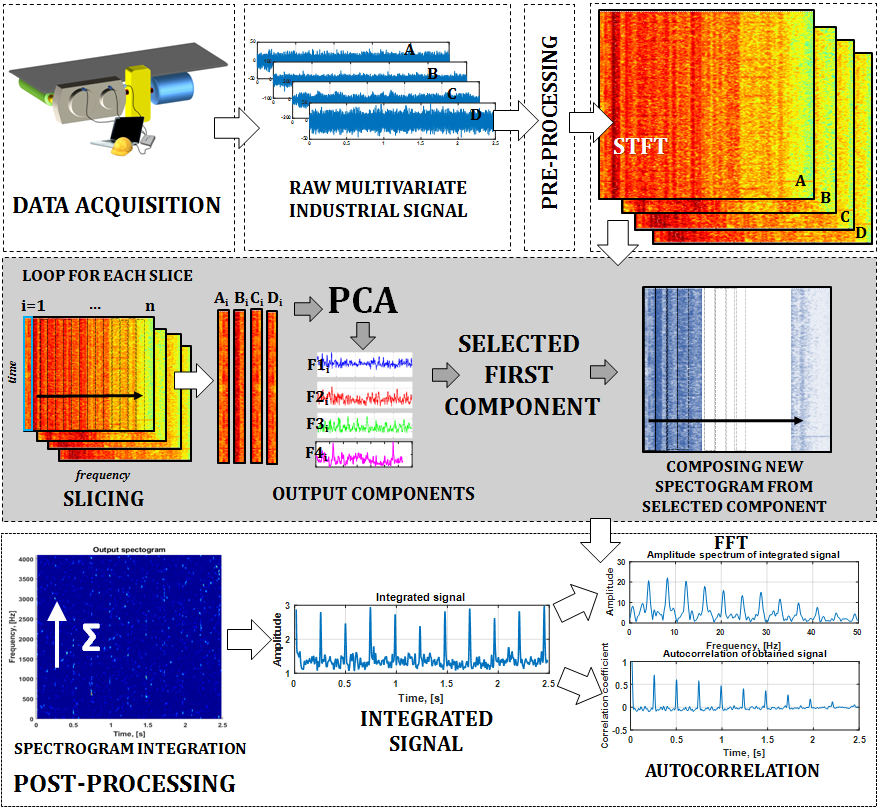
\includegraphics[width = \textwidth]{wykresy/pca_block.png}
\caption{Functional schematic of~presented method.}
\label{fig: pca_block}
\end{figure}


\newpage
\section{Methods for multidimensional domain analysis using NMF algorithms}

In this section, the~author describes techniques developed based on~the~factorization of~multidimensional data representations. In all described cases vibration signals are analyzed. From among many different multidimensional data representations two have been selected because of~their properties: spectrogram, which is~a~squared magnitude of~Short-Time Fourier Transform (STFT) and Cyclic Spectral Coherence (CSC). A~spectrogram is~a~time-frequency representation, and it~can be~interpreted in~two ways: either as~a~short-time Fourier spectrum that changes in~time or as~time-domain subsignals described in~narrow frequency bands within the~entire frequency spectrum of~the~input signal. CSC is~a~bi-frequency representation with two frequency axes describing nonlinear links between the~carrier frequency and modulating frequency. It can be~interpreted as~autocorrelation of~spectrogram matrix and provides information about cyclic modulations with respect to~the~carrier frequency domain.

General idea of~matrix factorization assumes that it~is~possible to~approximate a~matrix with two (or more) factors being (typically) lower-rank matrices (see Figure \ref{fig:met_nmf}). There is~a~lot of~different classes of~factorization algorithms, the~most popular being: Singular Value Decomposition (SVD) \cite{cempel2007multidimensional,cempel2008generalized}, Eigenvalue Decomposition (EVD) \cite{golub2012matrix,johnson1985matrix}, LU decomposition \cite{householder2013theory}, Cholesky decomposition \cite{golub2012matrix,johnson1985matrix} etc.

\begin{figure}[ht!]
\centering
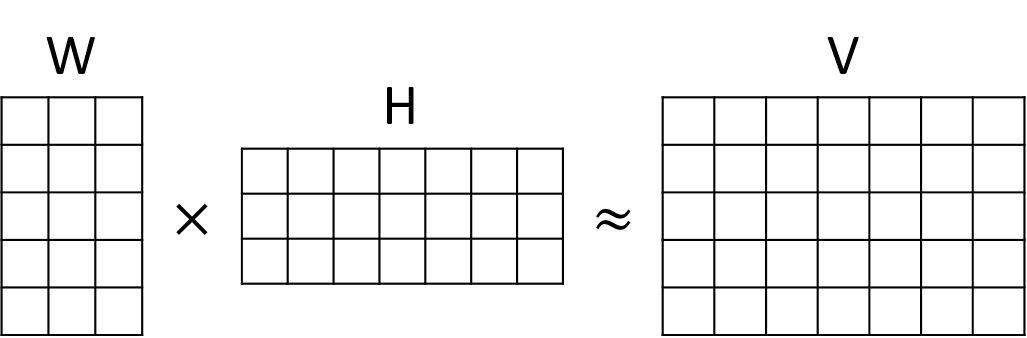
\includegraphics[width=0.8\textwidth]{wykresy/met_nmf.png}
\caption{General idea of~matrix factorization}
\label{fig:met_nmf}
\end{figure}

Each class of~algorithms can be~characterized with different properties, e.g. some only accept and return square matrices, others also produce third diagonal matrix, etc. NMF-type algorithms, on~the~other hand, have the~unique property of~only accepting and returning matrices with nonnegative entries. 


\subsection{STFT analysis taking advantage of~NMF encoding matrix}\label{met_nmf_enc}

In the~first case of~NMF-based method design author focuses on~the~utilization of~\emph{encoding matrix} (matrix H in~Figure \ref{fig:met_nmf}) generated by~NMF algorithm while factorizing spectrogram matrix of~vibration signal recorded on~the~damaged bearing of~the~belt conveyor's drive pulley. Flowchart of~the~described procedure is~presented in~Fig. \ref{fig:met_enc_nmf}.

In the~first step spectrogram matrix of~the~signal is~calculated according to~the~description in~section \ref{STFT} in~the~appendix. Then author used Semi-Binary NMF (see section \ref{ap_sbnmf} in~the~appendix) algorithm to~group spectra vectors across all timestamps of~the~spectrogram. Encoding matrix produced by~NMF carries information about the~timestamp occurrence within clusters, which allows constructing so-called “partial output spectrograms”. They are matrices of~zeros with appropriate spectra vectors distributed among them. As a~result of~this step, we obtain $J$ partial spectrograms where $J$ is~a~predefined number of~clusters. The inverse short-time Fourier transform (ISTFT) is~performed on~all of~them using built-in Matlab function \code{istft} \cite{benesty2007springer}, and the~one of~maximum kurtosis is~selected for further processing.

At this point obtained selected signal reveals presence at~correct timestamps of~impulses occurrence, but those areas do not look like impulses yet. To extract the~correct form of~the~impulses, highpass filtration is~required. It gets rid of~low-frequency high-energy frequency components and preserves impulse present in~a~wide band of~the~spectrum. The~procedure has been published in~\cite{wodecki2017local}.


\begin{figure}[ht!]
\centering
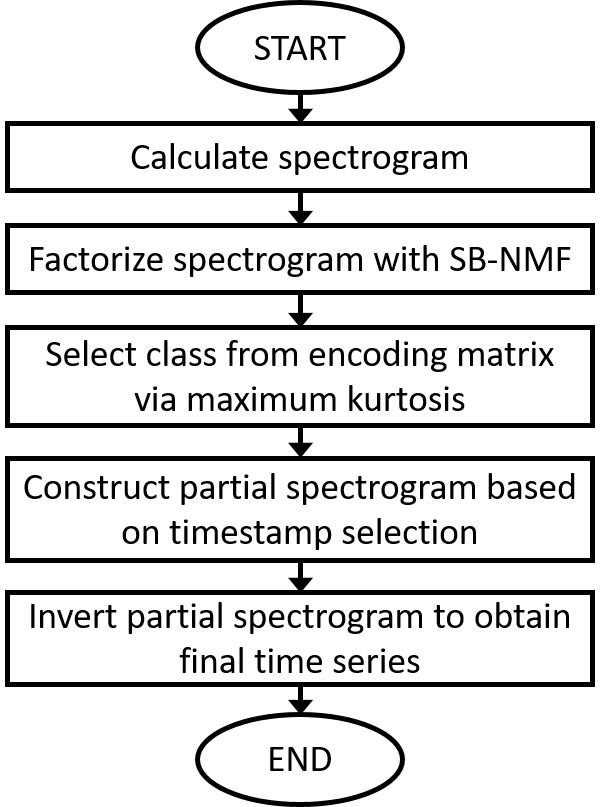
\includegraphics[width=.4\textwidth]{wykresy/met_enc_nmf.png}
\caption{Flowchart of~the~proposed procedure}
\label{fig:met_enc_nmf}
\end{figure}

\subsection{STFT analysis taking advantage of~NMF base matrix}\label{met_nmf_base}

In the~next case of~NMF-based method design author utilizes so-called \emph{base matrix} (matrix W in~Figure \ref{fig:met_nmf}) generated by~NMF algorithm while factorizing spectrogram matrix of~vibration signal recorded on~the~damaged bearing of~the~copper ore crusher. In that case base matrix produced by~NMF was used to~classify spectra vectors along the~time dimension. As a~result, the~filter characteristic is~designed, that allows isolating the~damage component. Flowchart of~the~described procedure is~presented in~Fig. \ref{fig:met_base_nmf}.

Firstly, the~signal has to~be transformed into a~time-frequency domain. For such transformation spectrogram has been chosen (see section \ref{STFT}). Considering it~as~nonnegative data matrix author applies NMF to~factorize spectrogram. In this context NMF is~used as~clustering tool group spectra vectors $\textrm{Spec}[f,\Delta t[i]]$, where $f$ denotes full Nyquist frequency domain for given data. Obtained spectrogram matrix $Spec$ will serve as~input matrix $\mathbf{V}$ for NMF factorization (see Eq. \ref{V1}). To perform the~factorization, the~author defines the~value $r$ as~the~rank of~factorization. Then NMF factorization is~performed to~obtain the~matrix \textbf{W} that will be~composed of~\textit{r} vectors - related to~clusters - that contain description of~spectral content of~each cluster $i=1 \dots r$. Each column vector of~\textbf{W} is~considered to~be averaged spectral density and can be~used as~filter characteristic (also named \emph{selector}).

Finally, the~input signal is~filtered with FIR filter, where the~given selector is~used as~filter frequency response \cite{alan1989discrete}. In~the~end, envelope spectra of~obtained signals are calculated to~inspect fundamental and harmonic frequencies of~the~components \cite{randall2011rolling}. Additionally, IFB can be~presented as~a~frequency band for which the~desired selector is~the~strongest of~the~whole bank. The~procedure has been published in~\cite{wodecki2017novel}.

\begin{figure}[ht!]
\centering
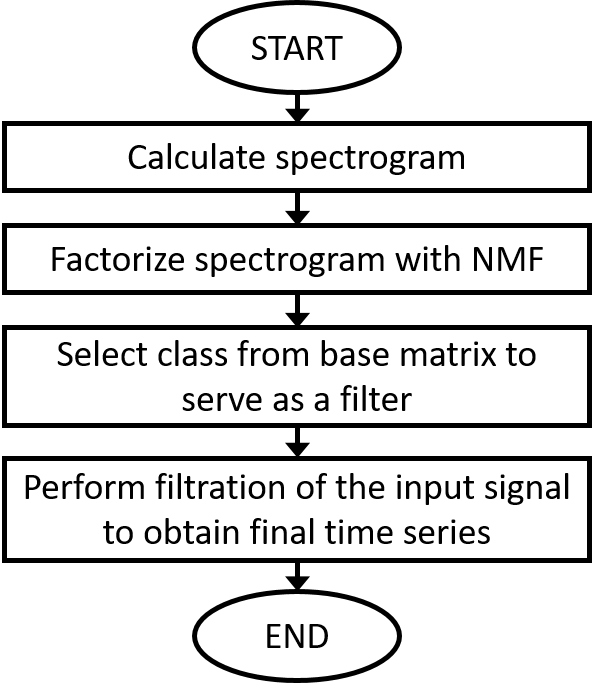
\includegraphics[width=.4\textwidth]{wykresy/met_base_nmf.png}
\caption{Flowchart of~the~proposed procedure}
\label{fig:met_base_nmf}
\end{figure}

\subsection{CSC analysis taking advantage of~complete NMF output}\label{met_nmf_both}

In this chapter author presents multistage processing methodology for fault identification in~rotating machinery scenario, however, it~is~suitable for the~case when the~other periodic impulsive component is~also present in~the~signal. The~flowchart in~Figure \ref{fig:met_mcnmf} presents the~outline of~the~proposed procedure.

\begin{figure}[ht!]
\centering
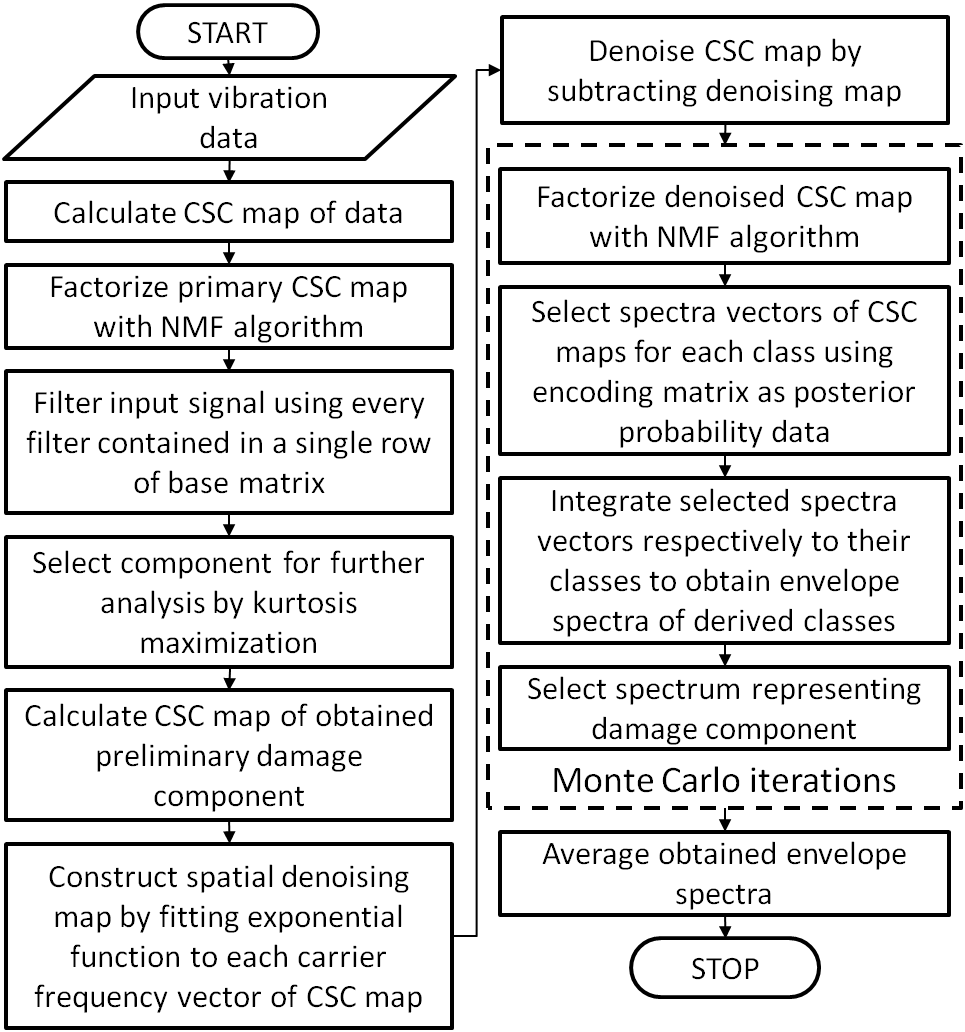
\includegraphics[width=.7\textwidth]{wykresy/met_mcnmf.png}
\caption{Flowchart of~the~proposed procedure}
\label{fig:met_mcnmf}
\end{figure}

The main idea is~focused on~utilizing all the~information that the~factorization algorithm can provide for such a~problem. Typically when NMF is~used, authors of~proposed methods are only interested in~the~information held by~one of~the~output matrices. One of~the~typical examples is~time-frequency map analysis \cite{wodecki2017local}, where authors use \emph{encoding matrix} to~classify spectra vectors in~the~time domain, allowing to~extract impulses from vibration data. While the~method is~effective, it~is~important to~note that the~\emph{base matrix} remains unused, leaving behind the~information that can still be~of~some value. Based on~this idea, the~author proposes to~utilize the~information from both output matrices in~a~sequential manner. 

Since the~input vibration signal has a~relatively complex structure in~terms of~the~presence of~cyclic components, instead of~time-frequency representation author decided to~use the~bi-frequency representation called Cyclic Spectral Coherence (CSC) as~a~basis for the~analysis (see section~\ref{app_csc} in~the~appendix). In the~first stage of~processing, CSC map is~firstly factorized with NMF algorithm (see section~\ref{app_nmf} in~the~appendix), and the~base matrix is~used as~a~set of~filters in~the~carrier frequency domain. Then, the~input signal is~filtered through a~selected filter, which results in~significant improvement of~the~signal in~terms of~SOI detectability \cite{wodecki2017novel}. 

In the~second stage of~processing obtained signal is~spatially denoised in~the~bi-frequency domain. In order to~achieve that, every vector of~full modulating frequency range within a~single carrier frequency bin is~modeled with a~decaying exponential function. This way it~is~possible to~construct a~spatial noise model in~the~form of~a~matrix with the~same dimensions as~the~CSC matrix. After subtracting noise model matrix from the~CSC map, the~latter becomes more clear and visibility of~damage-related frequency components is~improved.

In the~third stage, denoised CSC map is~again factorized with NMF algorithm within the~iterations of~Monte Carlo (MC) simulation \cite{metropolis1987beginning}. In each iteration damage-related envelope spectrum is~extracted, and after averaging final form of~the~envelope spectrum is~obtained.

\subsubsection{Multidimensional approach}

Analytical procedures incorporating various types of~multidimensional analysis very often focus on~features regarding only one of~the~dimensions of~considered data. Examples of~such approach contain e.g. frequency dimension of~spectrogram matrix (spectral selectors, spectral kurtosis~\cite{antoni2006spectral}), time dimension of~spectrogram matrix (cyclic impulses detection~\cite{kruczek2017cyclic}), modulation frequency domain of~bi-frequency map (fault frequency indication~\cite{kruczek2017multiple}) etc. 

In contrast to~such approach presented method takes advantage of~information extracted with respect to~both dimensions of~the~two-dimensional map being the~key subject of~analysis. In the~first stage, a~filter is~constructed based on~base matrix carrying information about the~carrier spectrum. The filter allows extracting one cyclic component from the~mixture of~two. In the~third stage, encoding matrix is~analyzed in~order to~obtain the~enhanced representation of~the~envelope spectrum of~the~fault component, that after post-processing reveals the~perfectly clean spectral structure of~the~fault.

\subsubsection{Spatial noise modeling}\label{denoise}

In order to~enhance the~efficiency of~NMF operation in~the~third stage of~analysis, quality of~the~CSC map can be~improved. To achieve this, the~author decided to~introduce preconditioning as~a~second step of~the~analysis. Noise levels across the~map are spatially modeled and subtracted from the~data for each $\Delta f$. 

The spatial context is~created by~analysis of~each carrier frequency bin $f = \left[f_1, \dots ,f_m \right]$ along the~modulating frequency dimension $\alpha = \left[\alpha_1, \dots ,\alpha_n \right]$. Each vector is~modeled specifically to~describe the~energy of~the~noise within this frequency band. However, to~avoid improper fitting, samples of~impulses are treated as~outliers among the~general shape of~decaying noise and rejected based on~data distribution. 

Denote single modulation vector from CSC map as~$C_i=\left|\hat{\gamma}_X(f_i,\alpha)\right|^{2}$ where $i \in 1, \dots, m$ and $\alpha = \left[\alpha_1, \dots ,\alpha_n \right]$. Author proposes to~define outlier cutoff threshold as~$99^{th}$ percentile for $C_i$ denoted as~$\hat{c}_{99}$ and defined as:

\begin{equation}
  P\left( C_i\leq\hat{c}_{99} \right)\geq 0.99.
\end{equation}

In such case it~is~possible to~exclude indices of~values higher than $\hat{c}_{99}$ from the~domain $\alpha$ and denote such modified domain of~$\alpha$ as~$\alpha_{mod}$, and respective background noise reference data originating from $\left|\hat{\gamma}_X(f_i,\alpha)\right|^{2}$ as~$\left|\hat{\gamma}_X(f_i,\alpha_{mod})\right|^{2}$ where $i \in 1, \dots, m$.

Considering described modeling conditions, each vector $\left|\hat{\gamma}_X(f_i,\alpha_{mod})\right|^{2}$ is~modeled with single-term exponential function using non-linear least squares method. Obtained parameters $a_i \in A$ and $b_i \in B$ (where $A$ and $B$ are vectors of~parameters for entire $f$ domain) of~exponential function allow then to~obtain the~noise model over a~modified domain $\alpha_{mod}$ for given $f_i$. Such modeled noise components are arranged into a~spatial noise map $N$ defined as~follows:

\begin{equation}
  N(i,\alpha_{mod})=a_i \exp \left( b_i \left|\hat{\gamma}_X(f_i,\alpha_{mod})\right|^{2}\right),
\end{equation}
that can be~subtracted from the~CSC map, effectively causing its denoising:

\begin{equation}
  \mathrm{CSC_d}= \left|\hat{\gamma}_X(f,\alpha)\right|^{2}-N,
\end{equation}
where $\mathrm{CSC_d}$ denotes denoised CSC map.
%  \newpage

% \begin{figure}[ht!]
% \centering
% 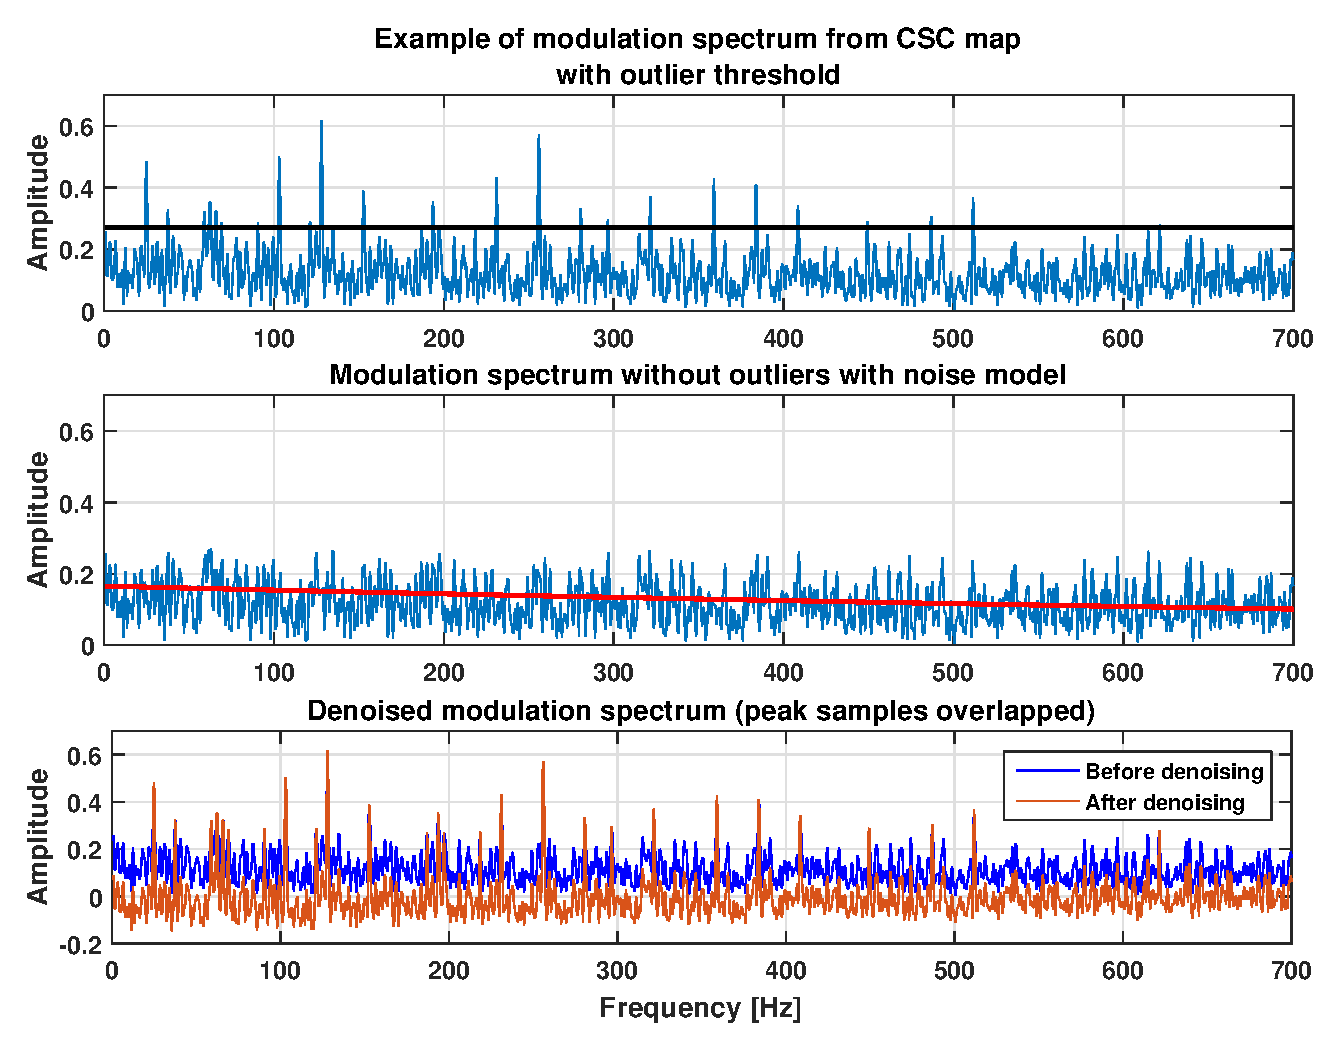
\includegraphics[width=.8\textwidth]{wykresy/ex}
% \caption{Example of~spatial denoising}
% \label{fig:ex}
% \end{figure}

\subsubsection{Monte Carlo simulation}\label{mcmc}

Monte Carlo (MC) methods are a~class of~algorithms that utilize random sampling in~numerical computation problems (see section \ref{app_monte}) \cite{metropolis1987beginning, metropolis1949monte}. The main idea is~to~use large-scale randomness to~discover deterministic behavior in~the~regarded problem. By the~law of~large numbers, the~expected value of~a~random variable can be~obtained approximately by~averaging independent samples of~the~variable using i.e. mean, median, etc. 

In the~presented application MC simulation is~used to~obtain good-quality envelope spectrum of~damage component in~the~diagnostic signal. In practice, the~role of~random sampling is~played by~calculating randomly initialized NMF of~denoised CSC map, using the~information provided by~obtained encoding matrix, and based on~that extracting envelope spectrum related to~local damage. Such spectrum will not be~exactly the~same in~every MC iteration, however, it~is~expected that most of~the~time outcome will be~mostly correct. Finally, averaging of~obtained results is~expected to~reveal true envelope spectrum related to~damage by~getting rid of~uncommon frequency components.

Within the~MC iterations, NMF is~used to~distinguish the~predefined amount of~groups $k$ of~different behavior to~be found in~denoised CSC map. Those groups are here called classes. As mentioned before, one of~them is~expected to~carry information about the~informative component related to~local damage. For the~interpretation of~obtained classes, the~author takes advantage of~the~encoding matrix operating in~the~domain of~modulating frequency. It is~easiest to~visualize this operation as~using posterior probability data (class indicator data) produced by~a~clustering algorithm. Encoding matrix can be~interpreted as~carrying information which class given point (here - given frequency component as~entire spectrum vector in~the~carrier domain integrated to~a~single value in~the~modulation domain) belongs to. Using this information it~is~possible to~construct the~envelope spectrum for each class. At this point, it~is~important to~be able to~automatically select the~cluster of~interest. It is~done by~calculating the~kurtosis value of~the~envelope spectrum vector for each class and selecting class with the~highest value. It is~motivated by~the~fact, that spectrum of~this class is~expected to~contain a~small number of~different frequency components, with the~majority of~zero values, while other classes will be~populated much more densely with frequency components carrying more coherent values of~energy. In this context, kurtosis value is~expected to~be highest for the~class related to~damage.

Finally, the~entire set of~envelope spectra obtained from MC iterations has to~be averaged to~obtain the~final result. Typically it~is~done using the~ordinary sample mean, however in~this application such an~approach would be~disadvantageous. Due to~random initialization of~NMF, in~most cases selected classes of~envelope spectra are expected to~contain a~small number of~improper frequency components in~the~notion of~false-positive result or, on~the~other hand, to~have expected correct frequency components missing. After using the~sample mean to~the~average large amount of~obtained spectra, those impurities of~the~first type (false-positives) will remain as~small values contaminating the~desired perfect spectrum after averaging. To avoid this effect, the~author used the~median function for averaging the~spectra. This way, unwanted contaminants will be~omitted, instead of~reduced.

As a~summary of~this section, single MC iteration is~constructed as~follows:

\begin{itemize}
  \item[$\bullet$] Factorize denoised CSC map with NMF;
  \item[$\bullet$] Use encoding matrix as~indicator data to~assign spectra vectors to~their respective classes;
  \item[$\bullet$] Integrate spectra vectors within each class placing them at~correct positions with respect to~the~modulating frequencies they stand for, which forms envelope spectra for all classes;
  \item[$\bullet$] Select class representing component of~interest.
\end{itemize}

\subsubsection{Kurtosis as~criterion for cluster selection}

In the~described application for every MC iteration, it~is~imperative to~be able to~automatically identify vector loosely populated with high-value nonuniform samples (highly non-Gaussian distribution) from among other vectors populated more densely with a~larger amount of~similar values (closer to~Gaussian distribution). In such context it~is~a~reasonable idea to~select vector with the~highest value of~kurtosis, which is~defined as~follows:

\begin{equation}
\label{eq:kurtosis}
Kurt[X]=\frac{m_4}{{m_2}^2}=\frac{\frac{1}{n} \sum_{i=1}^{n} \left(x_i - \overline{x} \right)^4}{\left({\frac{1}{n} \sum_{i=1}^{n} \left(x_i - \overline{x} \right)^2}\right)^2}
\end{equation}
where $m_4$ is~the~fourth sample central moment and $m_2$ is~the~second sample central moment (sample variance). The~procedure has been published in~\cite{wodecki2019impulsive}.


\newpage
\section{Automatic information extraction with Progressive Genetic Algorithm}\label{met_pga}

In this section author proposes novel method for vibration data analysis measured on~the~rolling bearing. In presented solution author pursues the~approach of~determining informative frequency band (IFB) of~the~signal, and hence extracting information about the~presence of~damage, that is~based on~optimal filtration. In practice, a~filter is~found, that is~dedicated to~optimally process the~given data. In opposition to~using classic adaptive filters \cite{makowski2014new,makowski2013procedure} or designing optimal filter prior to~predefined specification \cite{nilsson2003digital}, presented approach is~fully data-driven, and fitness function evaluates the~solutions only in~terms of~filtration performance. This way no functional constraints are imposed on~the~way that filter is~constructed by~the~evolution process. 

From mathematical point of~view, filter is~just an~equation of~discrete transfer function with $N$ coefficients (see eq. \ref{eq:fir}). For optimal filtering, both the~value of~$N$ and coefficients values should be~found. From such perspective, diagnostic methodology can be~considered as~multidimensional optimization problem. Genetic Algorithm (GA) is~one of~the~most frequently used tool for such task. However, it~should be~noted that presented procedure is~not a~simple application of~GA to~filter design. Author proposed a~complete progressive procedure for data-driven arbitrary filter development having no prior requirements. Kurtosis of~filtered signal is~used as~an~fitness value in~the~objective function, since local damage in~rotating machines presents itself as~wideband impulses in~vibration signal. However, an~original concept of~termination procedure is~proposed. In this work, progressive genetic algorithm has been applied for the~design of~linear phase digital FIR filter. Details of~ordinary GA operation can be~found in~the~appendix in~section \ref{GA}. The~procedure has been published in~\cite{wodecki2018optimal}.

\subsubsection{Filter encoding}

A~filter is~a~frequency selective object that allows a~certain frequency to~pass while attenuating the~others. Traditionally, different techniques exist for the~design of~digital filters. Of these, the~windowing method is~the~most popular \cite{alan1989discrete}. In this method, the~ideal impulse response is~multiplied with a~window function. There are various kinds of~window functions (Butterworth, Chebyshev, Kaiser, etc.), depending on~the~requirements of~ripples on~the~passband and stopband, stopband attenuation and the~transition width. These various windows limit the~infinite length impulse response of~ideal filter into a~finite window to~design an~actual response. However, windowing methods do not allow to~sufficient control of~the~frequency response in~the~various frequency bands and other filter parameters such as~transition width. The~user always has to~compromise on~one or the~other of~the~design specifications. So, evolutionary methods have been implemented in~the~design of~digital filters to~design with better parameter control. Since population-based stochastic search methods have proven to~be effective in~the~multidimensional nonlinear environment, all of~the~constraints of~filter design can be~effectively taken care of~by the~use of~these algorithms. 
Consider a~digital FIR filter with the~following transfer function:

\begin{equation}
\label{eq:fir}
\frac{x_n}{y_n}=a_0 + a_1 z^{-1} + a_2 z^{-2} +\dots +a_n z^{-n}
\end{equation}
where $\{a_1,\dots ,a_n \}$ are values of~the~filter coefficient vector. Since the~linear phase within the~passbands of~the~filter is~desired, the~author decided to~use symmetric coefficient vector with an~odd number of~coefficients. Such an~approach can also allow optimizing the~execution time since only one half of~the~coefficients has to~be evolved. The GA encoding of~a~filter is~a~string (chromosome), containing half of~the~coefficient vector $A=\{a_l,a_{l+1},a_{l+2},\dots,a_n\} \in \mathbb{R}$, where $a_l$ is~the~middle coefficient. Since FIR filters are inherently stable, there is~no need to~impose any search space constraints regarding zeros or poles on~the~\emph{Z} plane.

\subsubsection{Objective function}

Different types of~the~objective function can be~used for this kind of~problem \cite{mitchell1998introduction}. In this particular application, author follows the~approach of~impulsiveness maximization and ordinary kurtosis was used as~defined in~Eq. \ref{eq:kurtosis}.

It is~easy to~justify the~usage of~kurtosis. In case of~rotating machines, local damage reveals itself in~vibration signal as~wideband, typically periodic impulses. Since they cover a~wide range of~frequency spectrum, they are expected to~be short and sharp. It can be~anticipated that kurtosis will be~very susceptible to~those as~a~fitness function.

Fitness value plays the~role of~the~operator used by~the~genetic algorithm itself, however for visual inspection of~obtained IFB influencing the~signal structure, the~spectrogram is~used. 
The details of~spectrogram calculation are described in~the~appendix in~section \ref{STFT}

\subsubsection{Progressive GA} \label{pga}

The concept of~progressiveness of~genetic algorithm serves the~purpose of~the~robustness of~evolution. Let us assume that GA evolves whole, relatively long chromosome for a~given individual, right from the~beginning. This approach is~susceptible to~misdirected evolution. Since in~this application filter coefficients are evolved, long chromosome translates into a~large number of~coefficients, and this means that filter would be~able to~come out with relatively high precision. Since the~coefficient vector is~randomly initiated, high-precision filter evolution very often goes the~wrong way, and despite fulfilling the~condition of~the~increasing value of~the~fitness function, it~can be~lead to~local maximum, which difficult to~be fixed by~random mutation. 

To avoid this effect, the~author proposed to~start with a~short chromosome and increase its length every epoch that lasts the~predefined amount of~generations (of course unless it~will be~terminated by~stall limit constraint). It is~realized by~starting with the~short, very general filter at~the~beginning. The~first epoch is~expected to~optimize this filter, and since it~is~short, it~will capture the~general shape of~filter response, towards which the~evolution should proceed. Consecutive epochs extend the~previously optimized coefficients’ vector by~two additional random entries for each individual. This way filter precision gradually increases, with the~general direction of~evolution being preserved by~shorter filter optimized in~the~previous epoch.
Extensive testing shows that such an~approach results in~faster, more effective evolution. Utilization of~well-known test data to~be filtered proved, that local maxima are successfully avoided every time, which is~hardly ever the~case with evolving the~whole filter at~once.

\subsubsection{Global termination criterion}
Since PGA is~characterized by~several types of~irregular behavior such as~stepped fitness progression or negative peaks, it~is~difficult to~use any trivial, commonly used termination criteria like the~derivative of~fitness progression. This irregular behavior will be~explained in~section \ref{results_pga} using an~example of~the~real data analysis. To deal with such complex behavior, the~original idea of~PGA requires a~novel approach to~its termination. Hence, the~author proposes to~use normalized root mean square error (NRMSE) between fitness progression within a~single epoch, and its linear approximation. Error is~normalized to~statistic span of~the~fitness progression vector up to~a~given point, and its threshold is~set at~$5\%$:
\begin{equation}
\label{eq:spectrogram}
NRMSE(y_k,\hat{y_k})=\frac{1}{y(end) - y(1)}\sqrt{\frac{\sum_{i=1}^{n} \left(y_k - \hat{y_k} \right)^2}{n}}
\end{equation}
where $y_k$ is~the~fitness function segment of~$k^{th}$ epoch, $\hat{y_k}$ is~its linear fit obtained by~ordinary linear regression, $y(1)$ is~first value of~entire fitness vector, $y(end)$ is~the~current last value of~fitness vector, and \emph{n} is~the~length of~regarded segment.







